\documentclass[conference]{IEEEtran}
\IEEEoverridecommandlockouts
\usepackage{cite}
\usepackage{amsmath,amssymb}
\usepackage{graphicx}
\usepackage{booktabs}
\usepackage{multirow}
\usepackage{array}
\usepackage{float}
\usepackage{url}
\usepackage[hidelinks]{hyperref}
\graphicspath{{figs/}}
\newcommand{\ra}{$\rightarrow$}

\begin{document}

\title{From Static Coefficients to Learned Edge Weights:\\
Evidence-Based Kubernetes Attack-Path Analysis}

\author{\IEEEauthorblockN{Ganesh Daware (23BCS038), Gagan Rathod (23BCS106),\\
Venkatesh Dhangar (23BCS041), Advait Pathak (23BCS094)}
\IEEEauthorblockA{\textit{Department of Computer Science and Engineering}\\
\textit{Indian Institute of Information Technology Dharwad}, Dharwad, India}}

\maketitle

\begin{abstract}
Graph-based analysis of Kubernetes deployments, as proposed by Blaise and Rebecchi in \emph{Stay at the Helm}, correlates
configuration findings into an attack graph and reconstructs the most probable attack paths with Dijkstra's algorithm on
log-transformed edge probabilities. The node scores and edge probabilities in that work are predefined coefficients chosen by
the authors, and a single setting is evaluated. We present KubeAttackViz, an open-source implementation of the approach for live
clusters, and replace the predefined coefficients with evidence. We keep the paper's formulation, $w(e)=-\ln P(e)$, and obtain
$P(e)$ in one of two ways: steps decided by configuration (RBAC, NetworkPolicy, pod security) are proven from the live cluster
state, and vulnerability-exploitation steps use a gradient-boosting model trained on 361,825 NVD vulnerabilities labelled with
the CISA Known Exploited Vulnerabilities catalogue. On a temporal hold-out set, the model improves on the CVSS score from 0.770
to 0.887 ROC-AUC and from 5\% to 54\% precision in the top 100. Configuration edges agree with the API server on all 21,019
RBAC checks of a validation cluster. Against an answer key we did not write, the attack paths documented by the public projects
Kubernetes Goat and Bad Pods deployed unmodified, both weightings find all seven documented Goat attacks, but learned weights rank
them at a mean position of 2.5 instead of 17.5 among 80 paths and match 14 of 15 documented answers instead of 12. On three
live clusters, learned weights reorder attack paths (Spearman $\rho$ 0.57--0.84 against static coefficients), a cluster-admin
misconfiguration introduced at runtime is ranked first by learned weights but 17th by static ones, and the ranking is unchanged
for every value of the single remaining assumed parameter up to 0.3.
\end{abstract}

\begin{IEEEkeywords}
Kubernetes security, attack graphs, RBAC, exploit prediction, machine learning, CISA KEV, Dijkstra
\end{IEEEkeywords}

% ─────────────────────────────────────────────────────────────────────────────
\section{Introduction}
Kubernetes offers network segmentation, process isolation and role-based access control (RBAC), but these controls are
effective only when configured correctly. Helm Charts package the configuration into templates that can exceed 40,000
lines~\cite{blaise2022}. Auditing tools such as kube-bench, kube-hunter, Checkov, kubeaudit and Polaris check individual
settings, but they do not show how weaknesses combine into multi-step attacks.

Blaise and Rebecchi~\cite{blaise2022} address this gap with a four-step method: extract a graph from a Helm Chart, enrich it
with six security features, score nodes and edges against the Kubernetes threat matrix~\cite{mstm}, and reconstruct risky paths
with Dijkstra's algorithm. Their evaluation on 592 public Charts shows that missing network policies and pod affinities increase
the set of containers reachable from outside by a factor of 2.35.

The scores in~\cite{blaise2022} are \emph{predefined coefficients}: every severe vulnerability adds 1, running as root adds 100,
and a missing network policy gives an edge probability of 0.8. The authors evaluate one setting and do not study its effect.
The first version of our tool, KubeAttackViz~\cite{kav}, followed the same design. This paper asks whether these numbers can be
replaced by measured or learned probabilities, and what changes when they are. Our contributions are:
\begin{itemize}
\item an implementation of the graph method for live clusters, with the six features of~\cite{blaise2022} computed from API
objects and Pod Security Policies mapped to Pod Security Standards~\cite{pss};
\item an edge model that keeps the paper's $\log(1/z)$ formulation but takes $z$ from evidence: exact configuration checks, or a
CVE exploitation model trained on public data without synthetic labels;
\item validation of the predicted edges against a running cluster (22,425 checks);
\item an external benchmark: attack paths documented by Kubernetes Goat~\cite{goat} and Bad Pods~\cite{badpods}, deployed
unmodified, used as an answer key for both weightings;
\item a comparison of static and learned weights on three live clusters, a runtime drift experiment, and a sensitivity analysis
of the one assumed parameter.
\end{itemize}

% ─────────────────────────────────────────────────────────────────────────────
\section{Background and Related Work}
\subsection{Stay at the Helm}
Fig.~\ref{fig:method} summarises the method of~\cite{blaise2022}. A Chart is parsed into 16 resource categories; pods and
containers become vertices and pod-to-pod edges represent possible movement through missing network policies, permission to
execute in other pods, or co-location. Six features enrich the graph: container vulnerabilities (CVSS $>7$), pod accessibility,
security contexts and Pod Security Policies, RBAC permissions, network policies and pod affinities. A node receives a score per
threat-matrix tactic,
\begin{equation}
s(v)=\alpha_1 n_{\mathrm{vuln}}+\alpha_2 n_{\mathrm{cap}}+\textstyle\sum_k \beta_k\,\mathbb{1}[\mathrm{finding}_k(v)],
\end{equation}
and an edge receives a probability $z(e)$ from the $\gamma$ coefficients (Table~\ref{tab:coef}). The most probable acyclic path
maximises $\prod z(e)$; taking $\log(1/z(e))$ as the cost turns this into a shortest-path problem solvable by Dijkstra:
\begin{equation}
\pi^{*}=\arg\max_{\pi}\prod_{e\in\pi} z(e)=\arg\min_{\pi}\sum_{e\in\pi}\log\frac{1}{z(e)}.
\label{eq:dijkstra}
\end{equation}
A parameter $\omega$ gives a non-zero probability of reaching pods whose services are internal.

\begin{figure}[t]
\centering
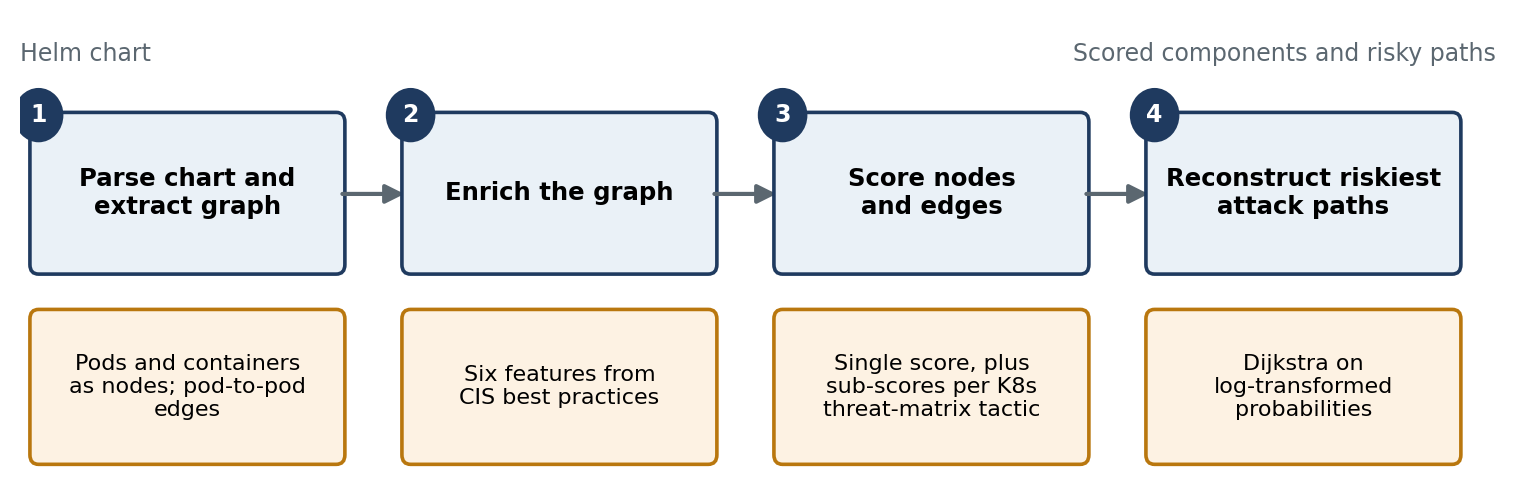
\includegraphics[width=\columnwidth]{method.png}
\caption{The four-step method of~\cite{blaise2022} (redrawn).}
\label{fig:method}
\end{figure}

\begin{table}[t]
\caption{Predefined Coefficients of~\cite{blaise2022} (Table VI, Condensed)}
\label{tab:coef}
\centering
\footnotesize
\begin{tabular}{@{}llr@{}}
\toprule
Symbol & Meaning & Value \\
\midrule
$\alpha_1,\alpha_2$ & per vulnerability; per extra capability & 1; 5 \\
$\beta_1,\beta_2$ & exposed service; runs as root & 100 \\
$\beta_3,\beta_5$ & privilege escalation; exec into pods & 100 \\
$\beta_4$ & permission per tactic & 10 \\
$\beta_6,\beta_7$ & host network; host paths & 100 \\
$\beta_8$ & per host volume type & 10 \\
$\gamma_1,\gamma_2,\gamma_3$ & no net. policy; affinity; pod exec & 0.8; 0.4; 1 \\
\bottomrule
\end{tabular}
\end{table}

The evaluation covers 592 Charts from 14 repositories (1,076 pods, 1,318 containers). Fig.~\ref{fig:cis} shows the CIS
benchmark~\cite{cis} findings and the growth of the reachable set from 134 to 315 containers. The authors list better
vulnerability analysis, automated remediation and prioritisation, and CI/CD integration as future work.

\begin{figure}[t]
\centering
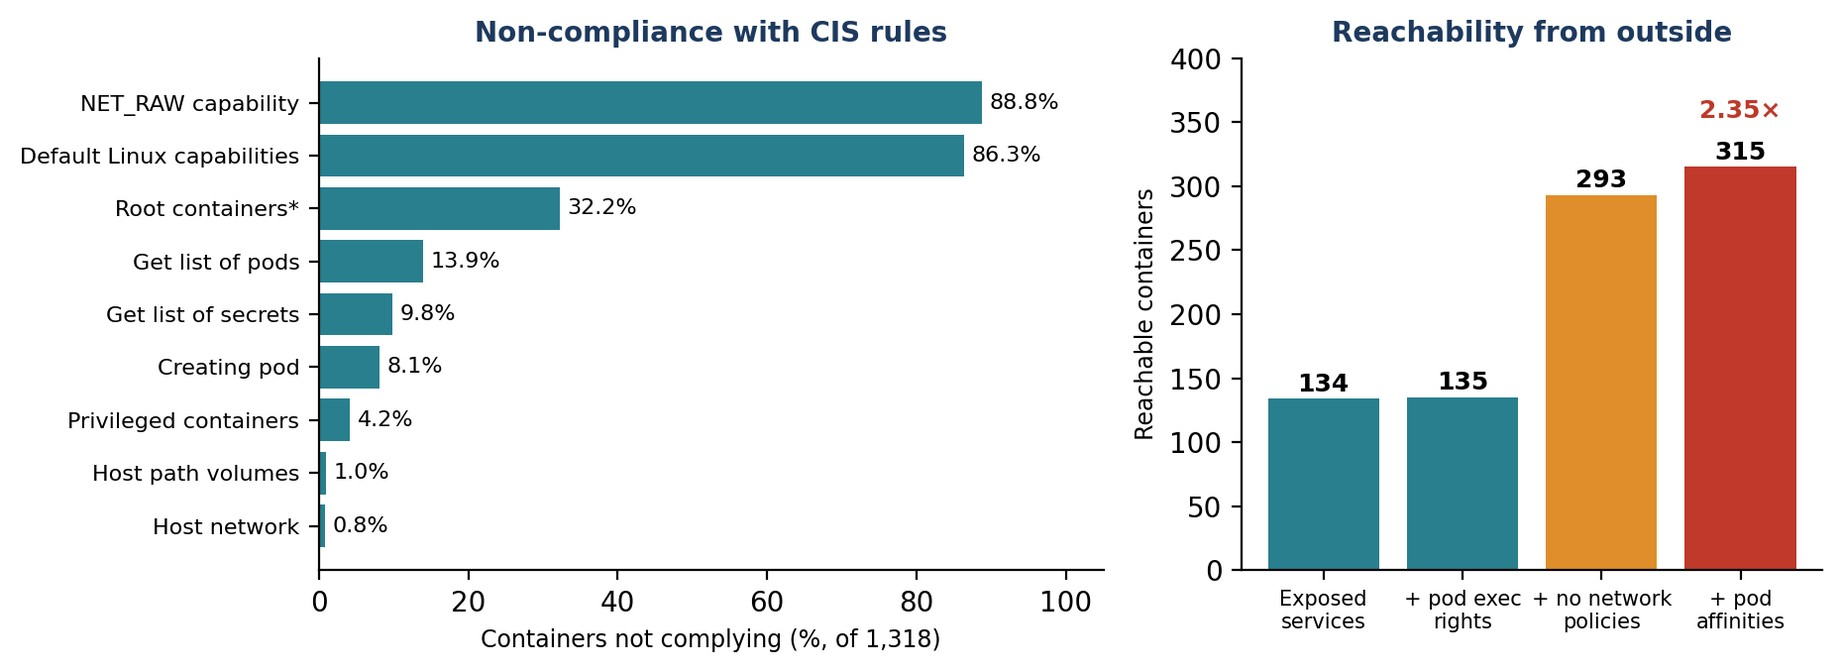
\includegraphics[width=\columnwidth]{cis_reach.png}
\caption{CIS non-compliance and reachability in the 592-Chart dataset, plotted from Tables IV and V of~\cite{blaise2022}.}
\label{fig:cis}
\end{figure}

\subsection{Limitations Addressed in This Work}
We identify four limitations of~\cite{blaise2022}: (L1) coefficients are chosen by hand and a single setting is evaluated;
(L2) vulnerabilities are \emph{counted}, so a hundred rarely exploited CVEs outweigh one actively exploited CVE; (L3) the
analysis is static and neither edges nor paths are checked against a running cluster or an external answer key; (L4) Pod Security Policies were removed in Kubernetes
v1.25~\cite{pss}.

\subsection{Related Work}
Attack graphs were generated automatically by model checking~\cite{sheyner2002} and from Datalog rules in
MulVAL~\cite{mulval2005}. CVSS~\cite{cvss} measures severity rather than likelihood of exploitation. EPSS~\cite{epss} predicts
exploitation in the next 30 days, and the CISA KEV catalogue~\cite{kev} lists vulnerabilities with confirmed exploitation. We use
KEV as ground truth and EPSS only as a reference. Kubernetes Goat~\cite{goat} is an intentionally vulnerable cluster whose
scenarios document attacks step by step, and Bad Pods~\cite{badpods} is a set of eight pod manifests whose documentation states
whether each gives root on the node. Neither was built to evaluate attack-graph tools, which makes them a neutral answer key.

% ─────────────────────────────────────────────────────────────────────────────
\section{System Design}
\subsection{Architecture}
KubeAttackViz (Fig.~\ref{fig:arch}) reads cluster state through \texttt{kubectl}, builds a directed graph of pods,
ServiceAccounts, roles, bindings, secrets and nodes with NetworkX, and runs BFS blast radius, Dijkstra attack paths, bounded
Johnson cycle enumeration, critical-node analysis and snapshot comparison. Entry points are Internet-exposed services, RBAC
users and explicitly labelled pods.

\begin{figure}[t]
\centering
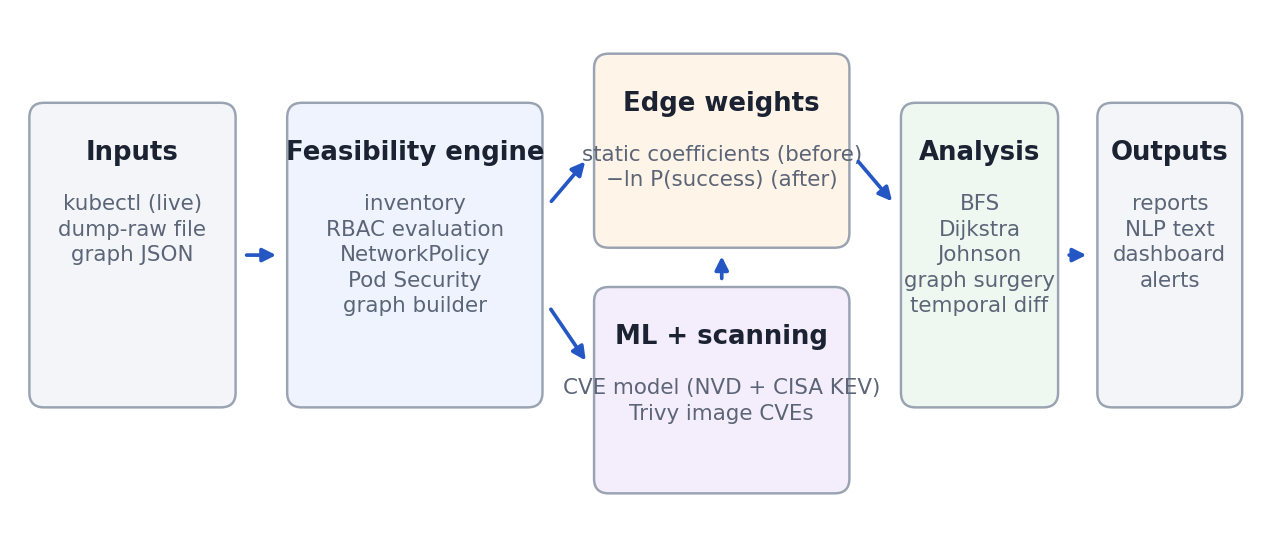
\includegraphics[width=\columnwidth]{arch.png}
\caption{KubeAttackViz architecture. The edge-weight stage is where static coefficients are replaced by probabilities.}
\label{fig:arch}
\end{figure}

\subsection{Feasibility Engine: the Six Features on a Live Cluster}
(1)~Every running image is scanned with Trivy~\cite{trivy}. (2)~NodePort and LoadBalancer services and Ingresses create
edges from an \emph{internet} source. (3)~Pod Security Standards (baseline) replace PSP checks: privileged mode, host namespaces,
hostPath, capabilities and root execution (L4). (4)~RBAC is evaluated fully: namespace scope, wildcards, \texttt{resourceNames},
ServiceAccount groups and token automount. (5)~NetworkPolicies are evaluated for ingress and egress with selector and port
semantics. (6)~Pods able to escape their container are linked to their node, which captures co-location.

\subsection{Baseline: Predefined Static Coefficients}
Like~\cite{blaise2022}, our first version assigned a fixed cost $c$ to each relation (e.g.\ \texttt{runs\_as} 2.0,
\texttt{can\_read} secret 3.0, \texttt{can\_exec} 3.5, \texttt{host\_access} 6.0) and a fixed impact $I$ to each node type.
Path risk was
\begin{equation}
\mathrm{risk}_{s}(\pi)=\frac{I(t)}{1+C(\pi)/10},\qquad C(\pi)=\textstyle\sum_{e\in\pi} c_{\mathrm{rel}(e)},
\end{equation}
with severity bands at 7, 5 and 3. These numbers are plausible but not measured (L1).

% ─────────────────────────────────────────────────────────────────────────────
\section{Learned Edge Weights}
\subsection{Edge Model}
We keep~(\ref{eq:dijkstra}) and change only the source of $z$. Each edge receives the probability $P(e)$ that the step succeeds:
\begin{equation}
w(e)=-\ln P(e),\qquad P(\pi)=\textstyle\prod_{e\in\pi}P(e)=e^{-\sum_{e\in\pi}w(e)},
\end{equation}
and path risk becomes $\mathrm{risk}_{\ell}(\pi)=I(t)\,P(\pi)$. Dijkstra's shortest path is thus the most likely path. We do
\emph{not} train a model to imitate our static coefficients, which would only reproduce them. Instead, each edge belongs to one
of three evidence classes (Table~\ref{tab:classes}). The scenario parameter $p_u$ plays the role of $\omega$ in~\cite{blaise2022}
and is the only assumed number in the model. Probabilities are clipped to $[0.01, 0.995]$ so that weights remain finite and
positive.

\begin{table}[t]
\caption{Evidence Classes for Edge Probabilities}
\label{tab:classes}
\centering
\footnotesize
\begin{tabular}{@{}>{\raggedright}p{0.17\columnwidth}>{\raggedright}p{0.43\columnwidth}>{\raggedright\arraybackslash}p{0.28\columnwidth}@{}}
\toprule
Class & Used for & $P(e)$ \\
\midrule
exact-config & RBAC grants, token mounts, network reachability, privileged pod \ra\ node & 0.995 if allowed; no edge otherwise \\
cve-model & exploiting a reachable workload & $1-(1-p_u)(1-p_x)$ \\
scenario & workload without known exploitable CVE; hostPath, hostPID, hostNetwork, hostIPC & $p_u=0.05$ \\
\bottomrule
\end{tabular}
\end{table}

\subsection{CVE Exploitation Model}
\emph{Data.} 361,825 CVEs from the NVD~\cite{nvd}, labelled positive when listed in CISA KEV (1,743 positives, catalogue
2026.11.09). No synthetic data is used.
\emph{Features.} CVSS base score and vector components, CWE, publication year, reference types (vendor advisory, exploit,
patch), vendor and product prevalence, and description keywords.
\emph{Model.} Histogram gradient boosting, compared with logistic regression and CVSS alone. To avoid leakage, we train on CVEs
published up to 2023 (179,970; 1,174 positive) and test on later ones (181,855; 569 positive). An image's probability is
\begin{equation}
p_x(\mathrm{image})=1-\textstyle\prod_{i}\left(1-\hat p_i\right).
\end{equation}

Severity alone is a weak signal: only 1.28\% of the 49,425 CVEs with CVSS 9--10 are in KEV. Within that band, the top model
quintile has a 5.5\% exploitation rate and the bottom quintile 0.01\% (Fig.~\ref{fig:cvss}), a distinction that a count-based
$\alpha_1$ cannot make (L2). Table~\ref{tab:ml} shows the temporal test results. Removing the phrase ``in the wild'' from
descriptions lowers ROC-AUC only to 0.876. EPSS scores better but uses post-publication exploit and telemetry data, so it is
shown only as a reference.

\begin{figure}[t]
\centering
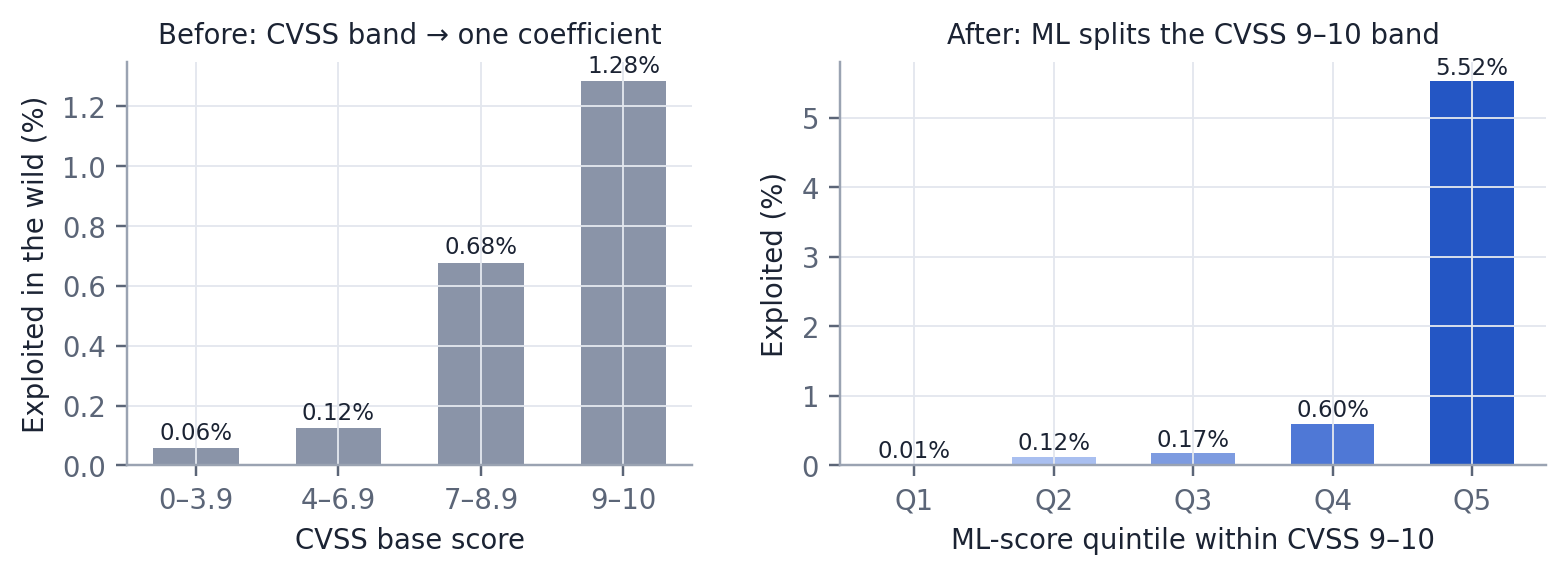
\includegraphics[width=\columnwidth]{cvss_vs_ml.png}
\caption{Left: KEV exploitation rate by CVSS band. Right: within CVSS 9--10, rate by quintile of the learned score.}
\label{fig:cvss}
\end{figure}

\begin{table}[t]
\caption{Exploitation Prediction on CVEs Published After 2023}
\label{tab:ml}
\centering
\footnotesize
\begin{tabular}{@{}lccc@{}}
\toprule
Model & ROC-AUC & PR-AUC & P@100 \\
\midrule
CVSS score only (baseline) & 0.770 & 0.012 & 5\% \\
Logistic regression & 0.877 & 0.112 & 48\% \\
\textbf{Gradient boosting (deployed)} & \textbf{0.887} & \textbf{0.108} & \textbf{54\%} \\
GB without ``in the wild'' & 0.876 & 0.097 & 42\% \\
EPSS (reference) & 0.975 & 0.428 & 89\% \\
\bottomrule
\end{tabular}
\end{table}

% ─────────────────────────────────────────────────────────────────────────────
\begin{figure*}[t]
\centering
\begin{minipage}[b]{0.49\textwidth}\centering
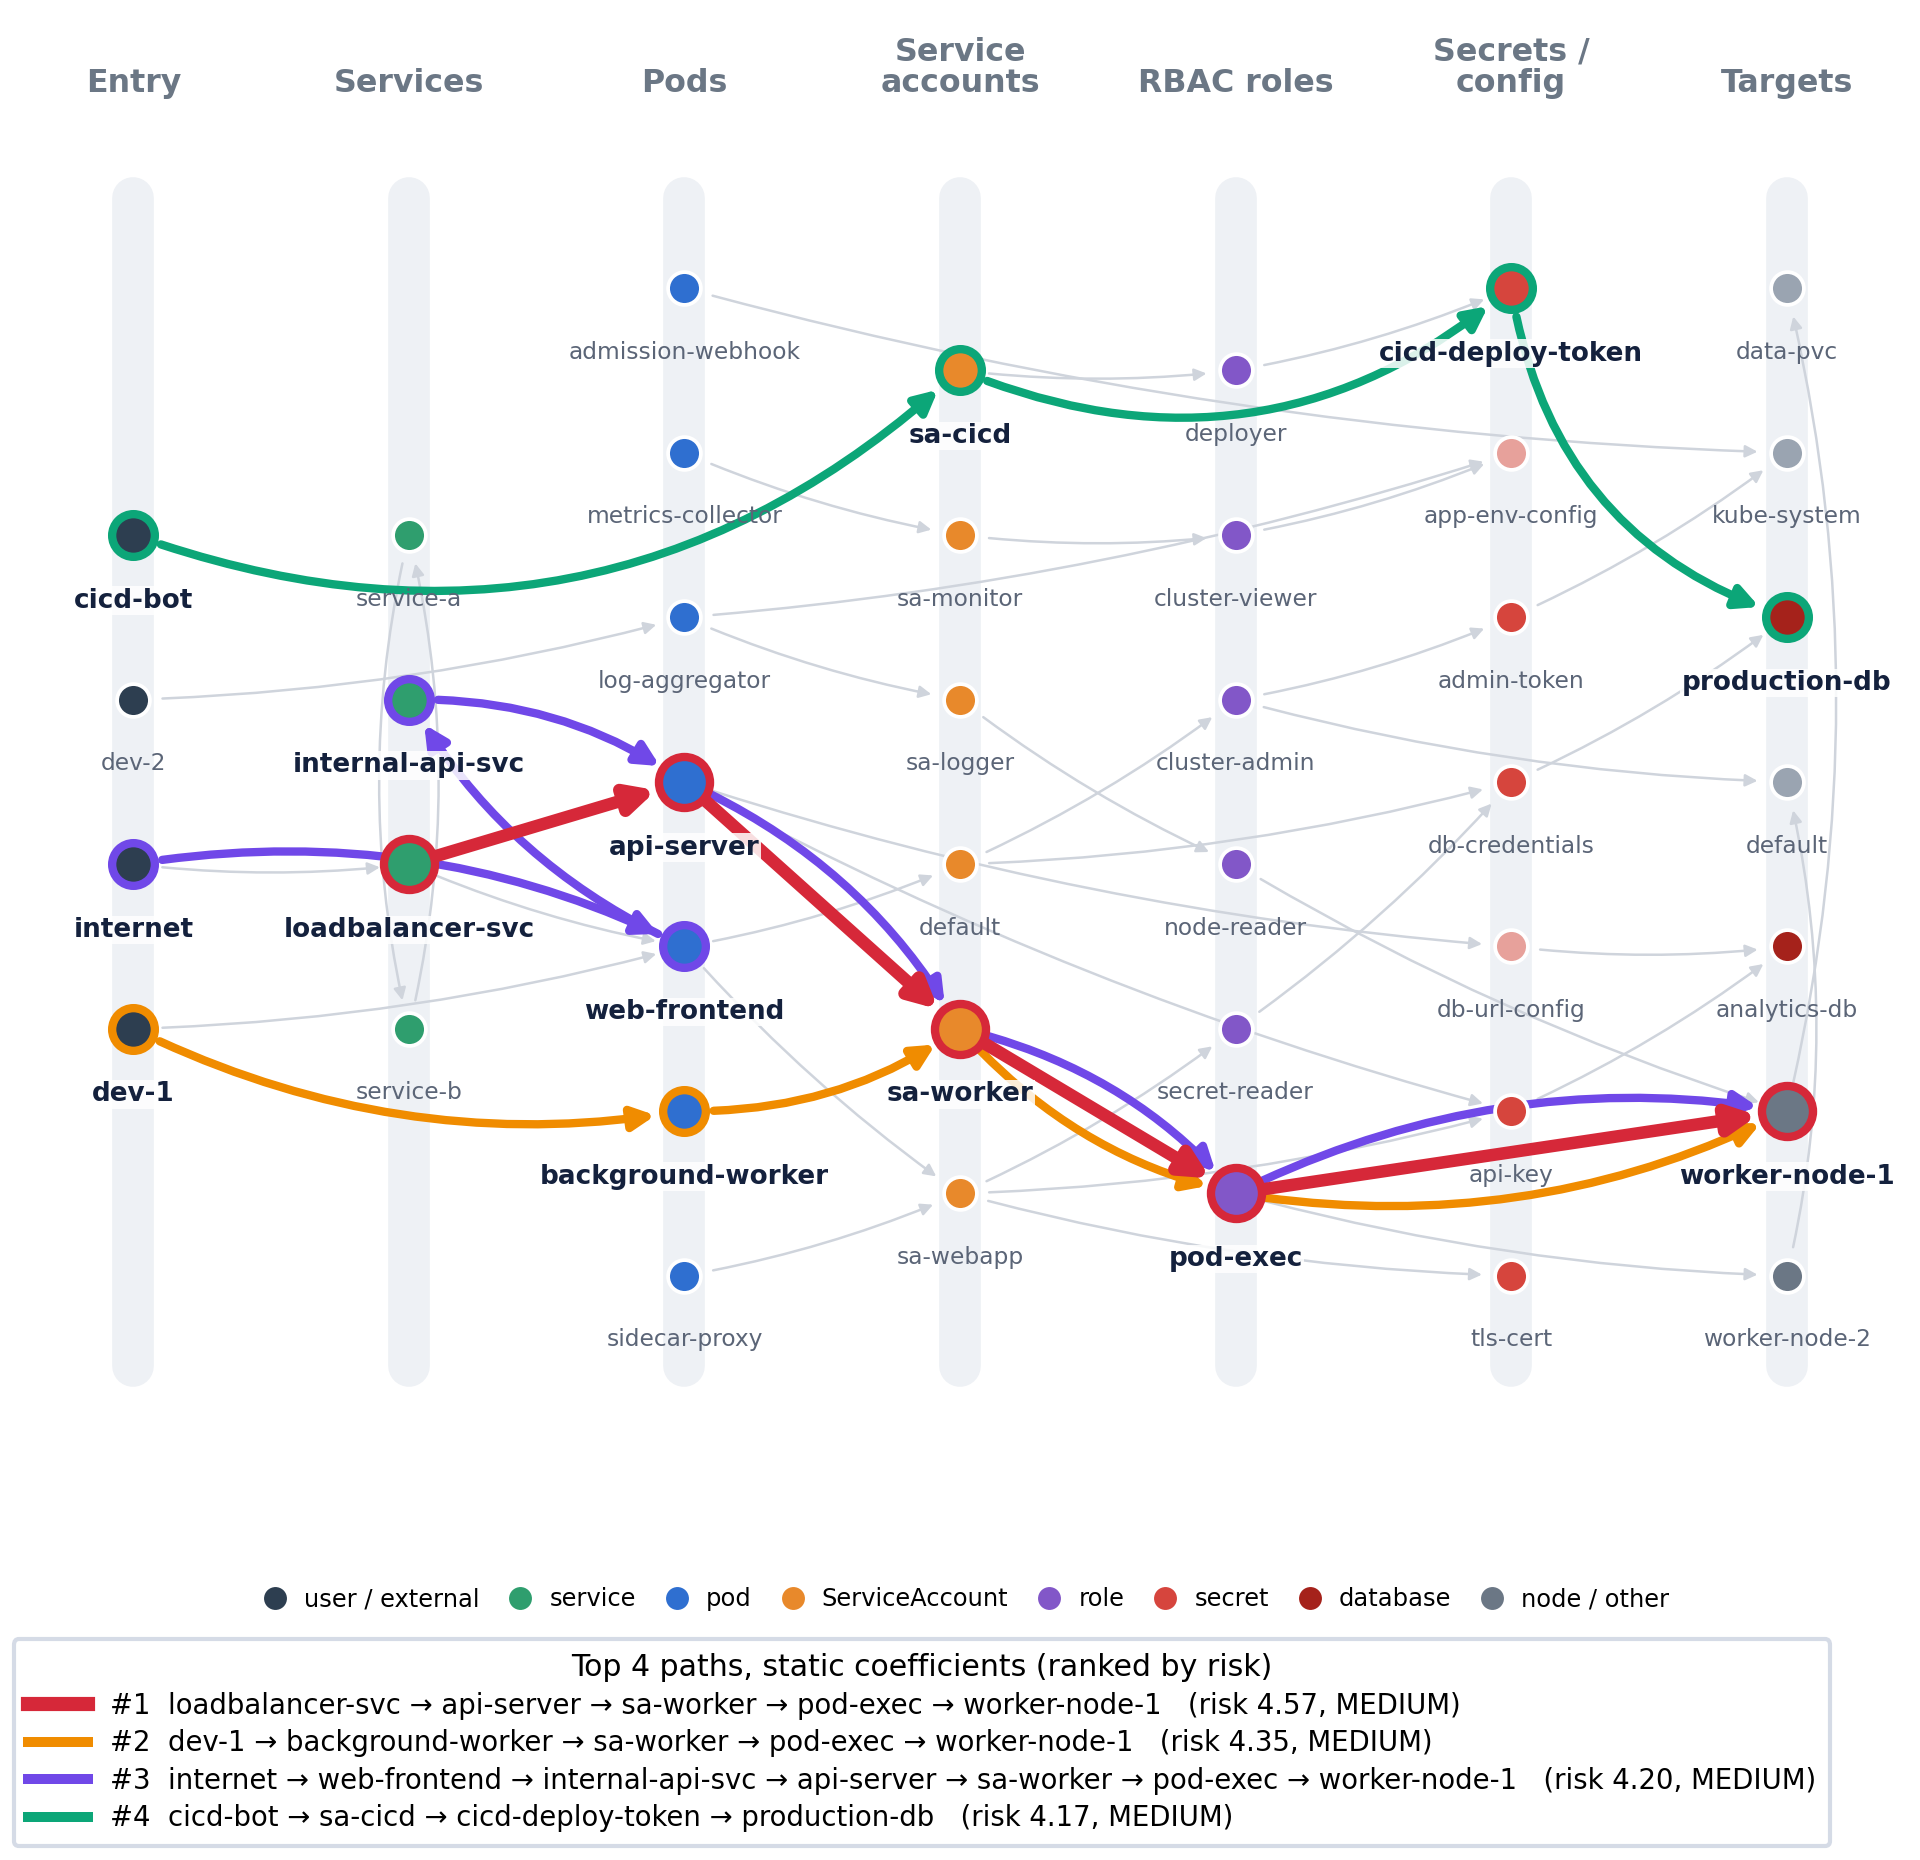
\includegraphics[width=\linewidth]{sample_static.png}\\[1pt]
{\footnotesize (a) First version: static coefficients}
\end{minipage}\hfill
\begin{minipage}[b]{0.49\textwidth}\centering
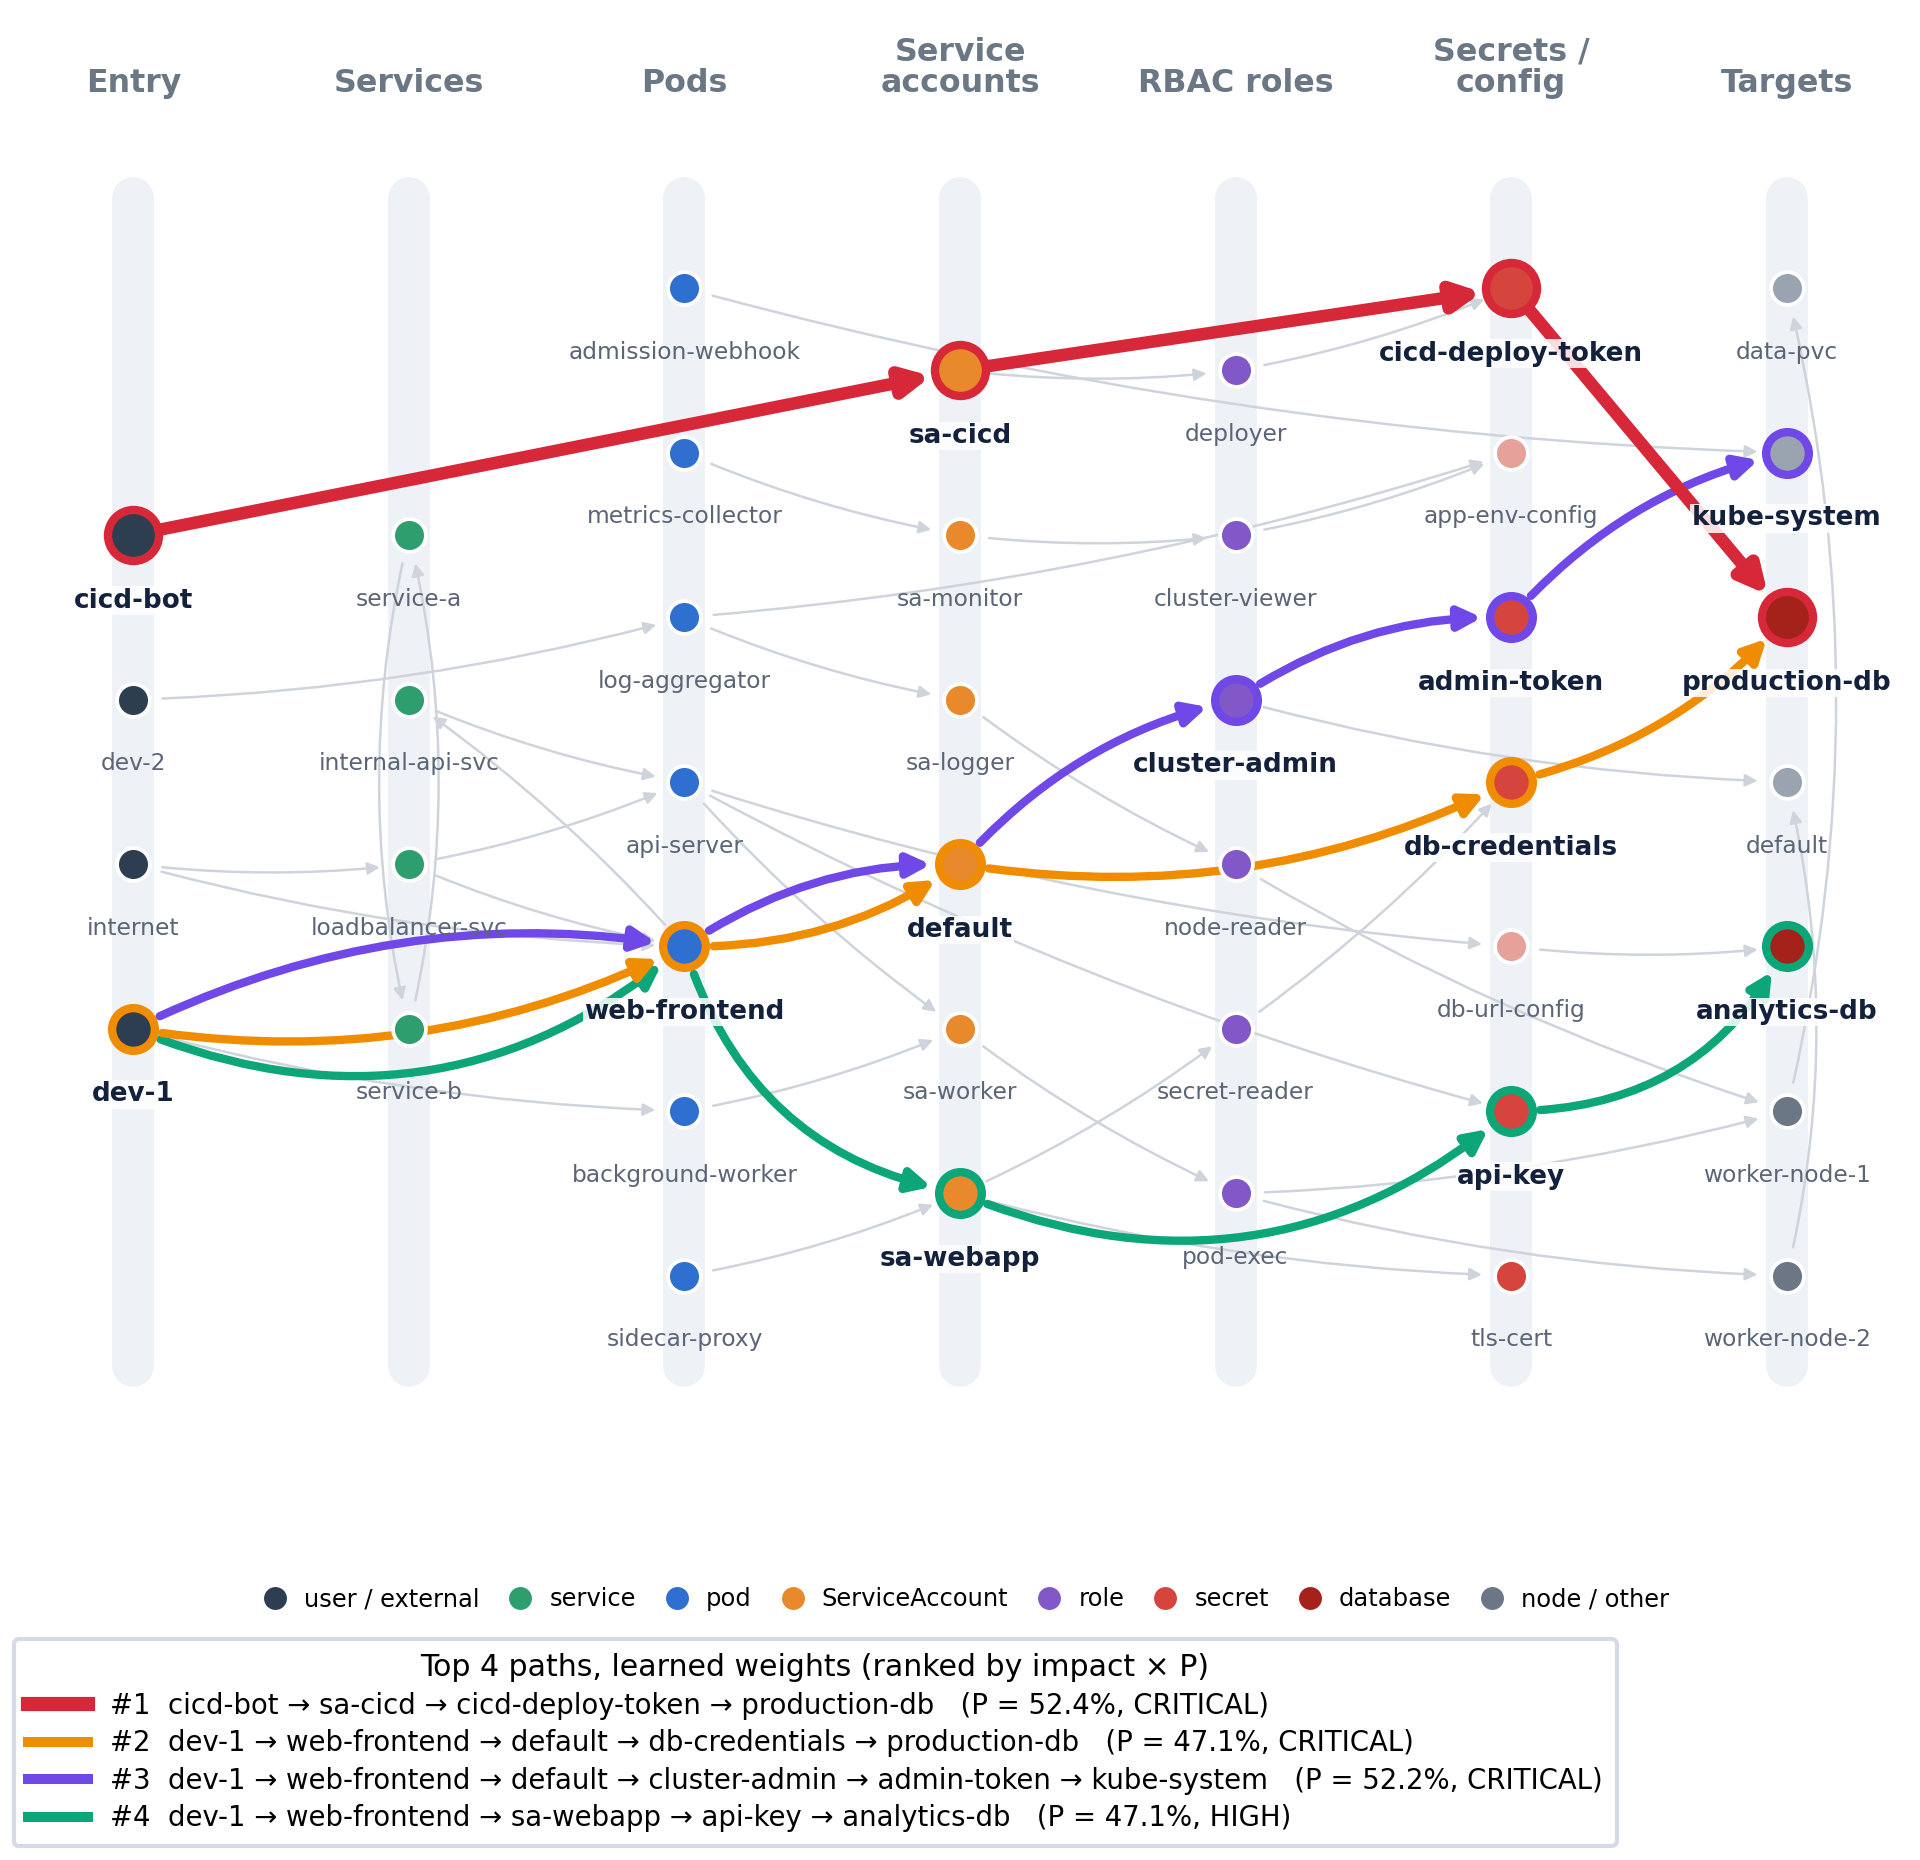
\includegraphics[width=\linewidth]{sample_learned.png}\\[1pt]
{\footnotesize (b) This work: learned weights}
\end{minipage}
\caption{The same 41-node sample cluster under both weightings, drawn with one layout (columns follow the attack chain from
entry points to targets); each panel highlights its four highest-ranked paths. (a)~With static coefficients all four are
MEDIUM, and three of them converge on \emph{sa-worker \ra\ pod-exec \ra\ worker-node-1}. (b)~With learned weights that node
chain drops out of the top four (the former \#1 falls to 15th, $P=0.7\%$); the top paths are the credential chain from
\emph{cicd-bot} to \emph{production-db} ($P=52.4\%$, formerly \#4) and three paths from \emph{dev-1} through
\emph{web-frontend} to production-db, kube-system and analytics-db. Three of the four are CRITICAL.}
\label{fig:beforeafter}
\end{figure*}

\begin{figure}[t]
\centering
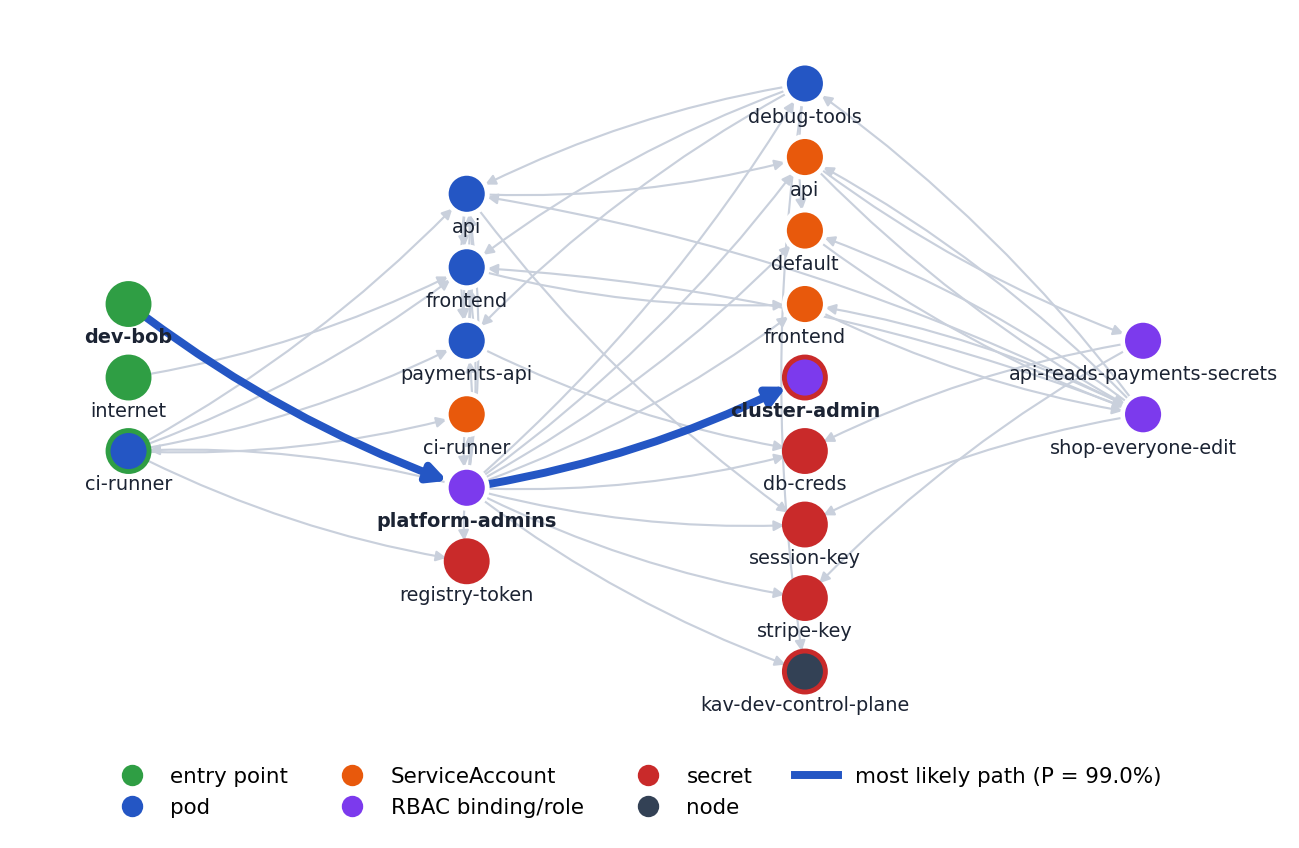
\includegraphics[width=\columnwidth]{devgraph.png}
\caption{Live dev attack graph, scoped to the 20 nodes on attack paths; the highlighted path is the most likely under learned
weights ($P=0.99$).}
\label{fig:dev}
\end{figure}

\begin{figure}[t]
\centering
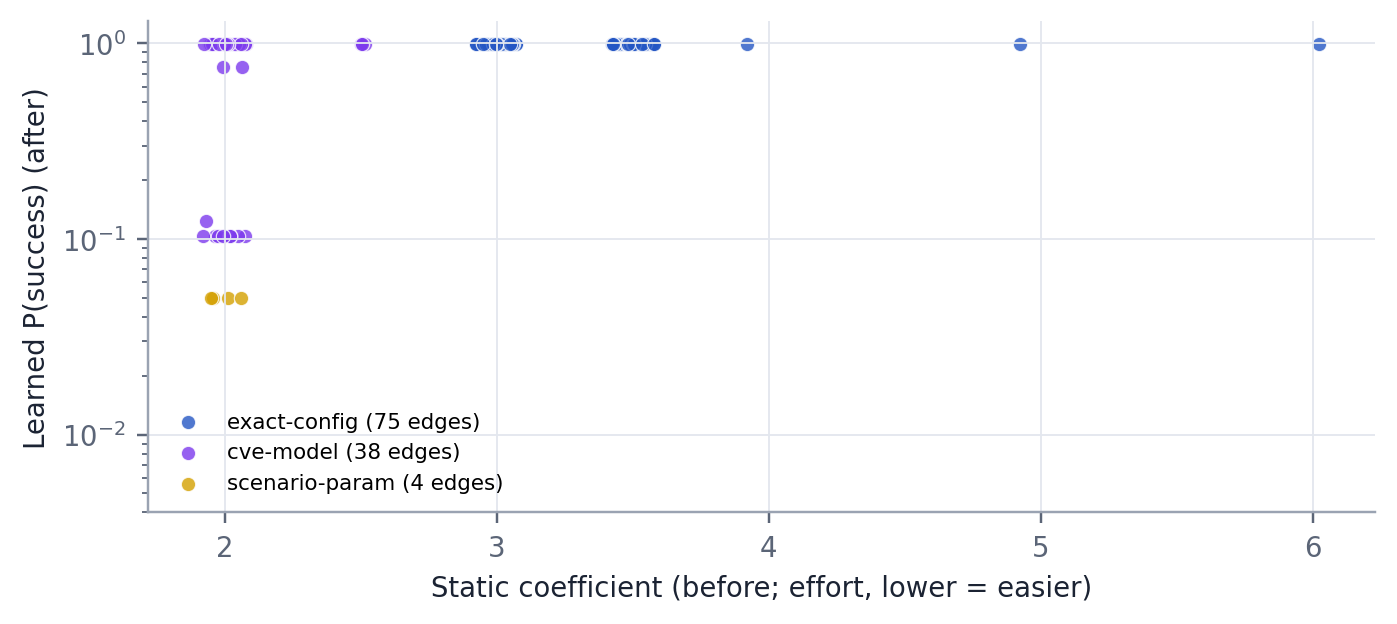
\includegraphics[width=\columnwidth]{edges.png}
\caption{Per-edge comparison on the three live clusters (117 edges): static coefficient (before) versus learned probability of
success (after, log scale), coloured by evidence class.}
\label{fig:edges}
\end{figure}

\section{Evaluation}
\subsection{Setup}
We built three monitored clusters (dev, staging, prod) and one validation cluster with kind v0.33.0 (Kubernetes v1.37.0,
kindnet CNI). They run realistic microservices (frontend, API, payments, checkout, ledger, Redis, a CI runner) with deliberate
misconfigurations of the kinds reported in~\cite{blaise2022}; prod additionally has network policies and hardened pods. Images
are scanned with Trivy v0.76.1. After scoping to application namespaces, each graph has 19--20 nodes. A fifth cluster,
bench, runs the unmodified Kubernetes Goat and Bad Pods manifests (26-node graph).

\subsection{Edge Validation on a Live Cluster}
To address L3, we deployed 26 scenarios on the validation cluster and compared every predicted edge with the cluster's answer:
SubjectAccessReview for RBAC, the mounted token for token edges, and HTTP probes between pods for network reachability
(Table~\ref{tab:lab}). All RBAC, token and ordinary network edges are exact. All 55 errors involve \texttt{hostNetwork} pods,
whose traffic NetworkPolicy does not govern consistently across plugins.

\begin{table}[t]
\caption{Predicted Edges Versus Live-Cluster Ground Truth}
\label{tab:lab}
\centering
\footnotesize
\begin{tabular}{@{}lrccc@{}}
\toprule
Check & $n$ & Prec. & Rec. & Acc. \\
\midrule
RBAC (SubjectAccessReview) & 21,019 & 1.000 & 1.000 & 1.000 \\
Token availability & 190 & 1.000 & 1.000 & 1.000 \\
Network, ordinary pods & 1,050 & 1.000 & 1.000 & 1.000 \\
Network, hostNetwork pods & 166 & 0.873 & 0.605 & 0.669 \\
\midrule
Overall & 22,425 & 0.996 & 0.982 & 0.998 \\
\bottomrule
\end{tabular}
\end{table}

\subsection{Public Benchmark: Kubernetes Goat and Bad Pods}
Edge validation checks single steps. To check whole paths without writing the answer key ourselves, we deploy the manifests of
Kubernetes Goat~\cite{goat} and Bad Pods~\cite{badpods} unmodified on the bench cluster (the one Goat component installed with
Helm is rendered from its default values; the Bad Pods get their own namespace). From Goat we take the seven scenarios whose
attack follows from configuration (2, 3, 4, 8, 11, 12, 16); the rest concern image contents, audit or runtime tools, or denial
of service. From Bad Pods we take all eight pods, whose documentation states whether the pod specification alone gives root on
the node. Following Goat's premise that any application can be compromised, entry points are the Internet, users and every pod,
giving 80 entry-to-target paths; risks are compared at two decimals, so ties share a rank. For Bad Pods, static weights have no
probability, so a modelled pod\ra node step counts as a claimed escape; learned weights claim one when $P\ge0.5$.

\begin{table}[t]
\caption{Kubernetes Goat Attacks: Found and Rank Among 80 Paths}
\label{tab:goat}
\centering
\footnotesize
\setlength{\tabcolsep}{3.5pt}
\begin{tabular}{@{}rlccc@{}}
\toprule
\# & Documented attack & Found & Static & Learned \\
\midrule
2 & Docker-in-Docker escape to host & \checkmark & \#20 & \textbf{\#1} \\
3 & SSRF to internal metadata-db & \checkmark & reach. & reach. \\
4 & container escape to host & \checkmark & \#20 & \textbf{\#1} \\
8 & NodePort exposes internal service & \checkmark & reach. & reach. \\
11 & namespace bypass to cache-store & \checkmark & reach. & reach. \\
12 & vault key from pod environment & \checkmark & \#1 & \textbf{\#1} \\
16 & SA token reads secrets (RBAC) & \checkmark & \#29 & \textbf{\#7} \\
\midrule
\multicolumn{2}{@{}l}{Mean rank of ranked attacks} & 7/7 & 17.5 & \textbf{2.5} \\
\bottomrule
\end{tabular}
\\[2pt]{\scriptsize ``reach.'': target is a workload, so the path is checked but not ranked.}
\end{table}

\begin{table}[t]
\caption{Bad Pods: Does the Pod Spec Reach Its Node?}
\label{tab:badpods}
\centering
\footnotesize
\setlength{\tabcolsep}{3.5pt}
\begin{tabular}{@{}rlcccc@{}}
\toprule
\# & Pod & Documented & Static & Learned & $P$ \\
\midrule
1 & everything allowed & esc. & esc. & esc. & 0.995 \\
2 & privileged + hostPID & esc. & esc. & esc. & 0.995 \\
3 & privileged & esc. & esc. & esc. & 0.995 \\
4 & hostPath & esc. & esc. & \underline{no} & 0.050 \\
5 & hostPID & no & \underline{esc.} & no & 0.050 \\
6 & hostNetwork & no & \underline{esc.} & no & 0.050 \\
7 & hostIPC & no & \underline{esc.} & no & 0.050 \\
8 & nothing allowed & no & no & no & 0.000 \\
\midrule
\multicolumn{3}{@{}l}{Agree with documentation} & 5/8 & \textbf{7/8} & \\
\bottomrule
\end{tabular}
\\[2pt]{\scriptsize Underlined: disagrees with the Bad Pods documentation.}
\end{table}

\begin{figure}[t]
\centering
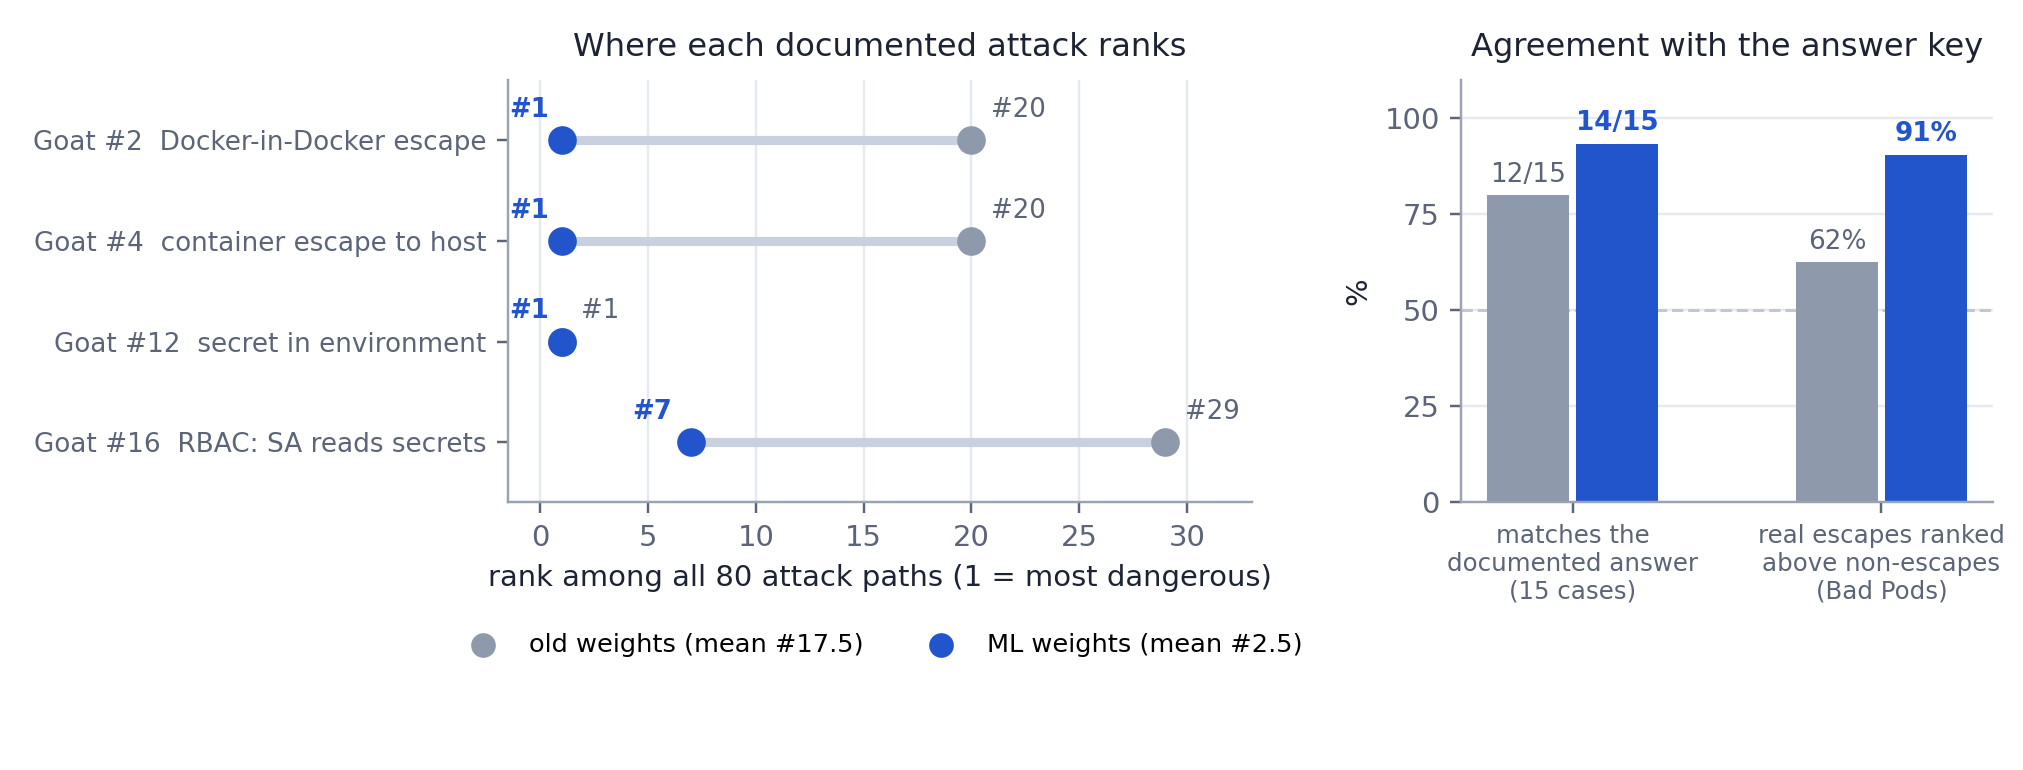
\includegraphics[width=\columnwidth]{benchmark.png}
\caption{Benchmark summary. Left: rank of each ranked Goat attack. Right: agreement with the 15 documented answers, and the share
of (escape, non-escape) Bad Pod pairs ordered correctly (dashed: chance).}
\label{fig:bench}
\end{figure}

Both weightings find all seven Goat attacks (Table~\ref{tab:goat}): weights change the order of paths, not which edges exist.
The difference is the ranking. Learned weights rank three of the four ranked attacks first and the fourth seventh, against 20th,
20th, 1st and 29th with static weights; the seventh place reflects that Goat's images contain KEV-listed CVEs, so many
``compromise a pod through a known-exploited CVE'' paths score almost equally. On Bad Pods (Table~\ref{tab:badpods}) static
weights give every pod with any host setting the same pod\ra node edge and so report hostPID, hostNetwork and hostIPC as
escapes, against the documentation. Learned weights treat privileged pods as configuration-decided and other host settings as
uncertain, matching seven of eight pods and ordering real escapes above non-escapes in 91\% of pairs (static: 62\%,
Fig.~\ref{fig:bench}). The one disagreement is hostPath: Bad Pods documents that mounting the host root gives the node, while
our model rates every hostPath mount at $p_u$; we report the miss rather than adjust the model after seeing the answer key.
Overall, learned weights match 14 of 15 documented answers and static weights 12.

\subsection{Static Versus Learned Weights}
Both weightings were applied to the same graphs (Table~\ref{tab:cmp}, Fig.~\ref{fig:sev}). The path rankings differ
substantially, most in prod ($\rho=0.57$). With static coefficients the one-edge path \emph{ci-runner \ra\ registry-token}
ranks first in every cluster because it is short. With learned weights the top path in dev is \emph{dev-bob \ra\
platform-admins \ra\ cluster-admin} (Fig.~\ref{fig:dev}): each step is a verified RBAC grant, so it succeeds with probability
0.99 and yields full cluster control. In prod, the break-glass role of \emph{sre-carol} reaches ledger and payment credentials
with probability 0.985 and moves up, while the network chain \emph{ci-runner \ra\ frontend \ra\ api \ra\ session-key}, ranked
second by the static model, drops because its pod-to-pod exploitation steps have low measured probability. Severity also gains
a meaning: a CRITICAL path reaches a high-impact target with high, evidence-backed probability, and the seven LOW paths in prod
depend on exploiting images with low measured exploitation probability.

Fig.~\ref{fig:edges} explains the reordering at the level of single edges. Static coefficients lie in a narrow band (2--6) and say nothing about whether a step will work. Learned probabilities separate into clear groups: configuration-proven edges at 0.995, exploitation edges whose images contain likely-exploited CVEs near 1, and exploitation edges with only unlikely CVEs near 0.1 or at $p_u=0.05$. Edges with the same static coefficient (about 2) can therefore differ by a factor of 20 in probability. Fig.~\ref{fig:beforeafter} shows the effect on the same sample cluster: with static coefficients all 18 paths are rated MEDIUM or LOW, while with learned weights three paths that end at production-db or kube-system become CRITICAL, and each path carries its probability of success.

\begin{table}[t]
\caption{Static Versus Learned Weighting on Three Live Clusters}
\label{tab:cmp}
\centering
\footnotesize
\setlength{\tabcolsep}{3.5pt}
\begin{tabular}{@{}lccllc@{}}
\toprule
Cluster & Nodes/edges & Paths & Static (C/H/M/L) & Learned (C/H/M/L) & $\rho$ \\
\midrule
dev & 20/51 & 16 & 0/13/3/0 & 16/0/0/0 & 0.71 \\
staging & 19/38 & 11 & 0/8/3/0 & 8/0/3/0 & 0.84 \\
prod & 19/28 & 19 & 0/5/14/0 & 4/0/8/7 & 0.57 \\
\bottomrule
\end{tabular}
\end{table}

\begin{figure}[t]
\centering
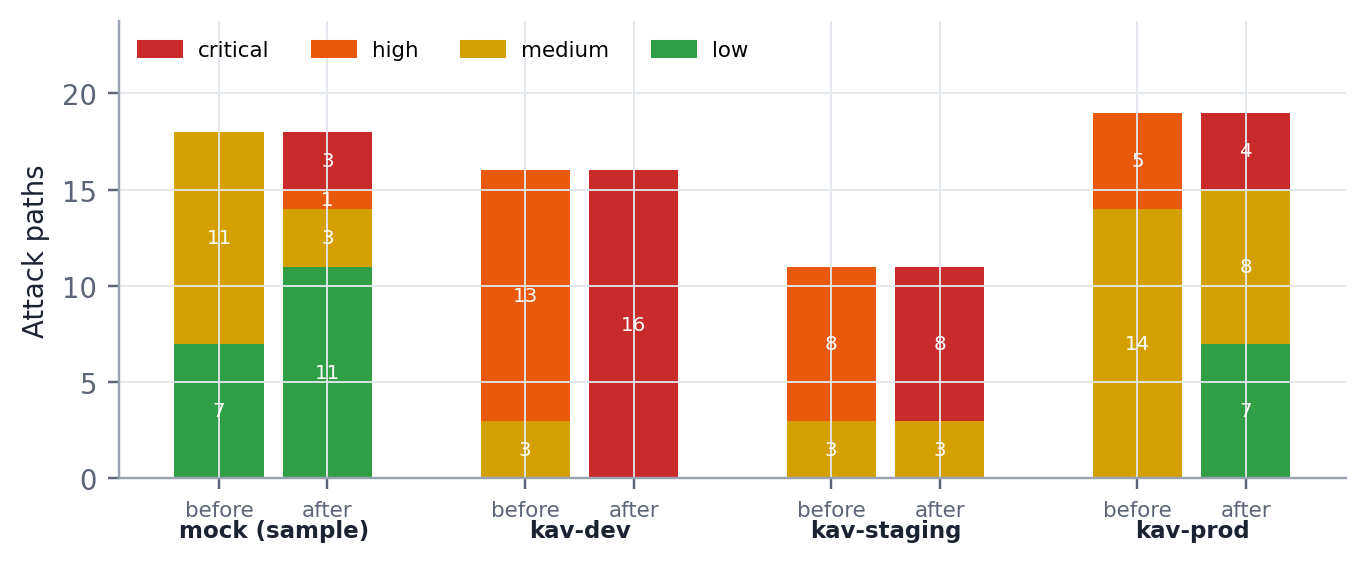
\includegraphics[width=\columnwidth]{sev.png}
\caption{Path severities before (static) and after (learned). ``mock'' is the sample cluster shipped with the tool.}
\label{fig:sev}
\end{figure}





\subsection{Sensitivity Analysis}
To address L1 for our own model, we varied $p_u$ from 0.01 to 0.5 and computed the Kendall $\tau$ of each cluster's path ranking
against the default $p_u=0.05$ (Table~\ref{tab:sens}). The ranking is identical for all $p_u\le0.3$ and the top path never
changes; only at $p_u=0.5$, which assumes half of all apparently unvulnerable services are exploitable, do some lower-ranked
paths swap.

\begin{table}[t]
\caption{Kendall $\tau$ of Path Rankings Against $p_u=0.05$}
\label{tab:sens}
\centering
\footnotesize
\begin{tabular}{@{}lccccccc@{}}
\toprule
$p_u$ & 0.01 & 0.02 & 0.05 & 0.10 & 0.20 & 0.30 & 0.50 \\
\midrule
dev & 1 & 1 & 1 & 1 & 1 & 1 & 0.962 \\
staging & 1 & 1 & 1 & 1 & 1 & 1 & 0.990 \\
prod & 1 & 1 & 1 & 1 & 1 & 1 & 1 \\
\bottomrule
\end{tabular}
\end{table}

\subsection{Runtime Drift}
The analysis in~\cite{blaise2022} runs once, before deployment. KubeAttackViz re-scans each cluster every 15\,s and compares
snapshots. While monitoring the hardened prod cluster we bound the ServiceAccount of its frontend pod to \texttt{cluster-admin}.
The change was detected after 16\,s with CRITICAL alerts, and the graph grew from 19 to 21 paths. The new path \emph{ci-runner
\ra\ frontend \ra\ cluster-admin} (via a deploy RoleBinding and the new binding) ranked first with learned weights ($P=0.975$,
CRITICAL) but 17th with static weights (MEDIUM), because it is long although every step is a verified grant. Removing the
binding was detected after 12\,s.

% ─────────────────────────────────────────────────────────────────────────────
\section{Discussion}
Table~\ref{tab:summary} compares the two approaches. The graph formulation and the log-probability search come
from~\cite{blaise2022}; our contribution is the source of the probabilities and the validation of the edges.

\emph{Threats to validity.} Our live comparison uses three small clusters that we built, so it shows how weighting changes
rankings rather than how frequent misconfigurations are; the 592-Chart dataset of~\cite{blaise2022} remains the reference for
prevalence. The public benchmark has 15 documented cases; it lists the attacks its authors designed, so we report recall and
rank rather than precision, and ranking documented attacks highly assumes they are among the most dangerous in their cluster.
The learned model rates every hostPath mount as uncertain, which disagrees with Bad Pods for a writable mount of the host root.
KEV lists only confirmed exploitation, so absolute probabilities are conservative; ranking metrics are less
affected. Multiplying probabilities assumes independent steps, as in~\cite{blaise2022}. Reachability of hostNetwork pods is not
modelled exactly.

\begin{table}[H]
\caption{Stay at the Helm Versus KubeAttackViz}
\label{tab:summary}
\centering
\footnotesize
\begin{tabular}{@{}>{\raggedright}p{0.2\columnwidth}>{\raggedright}p{0.32\columnwidth}>{\raggedright\arraybackslash}p{0.36\columnwidth}@{}}
\toprule
Aspect & Stay at the Helm~\cite{blaise2022} & KubeAttackViz (learned) \\
\midrule
Input & Helm Charts & live clusters, monitored \\
Edge weight & $\log(1/z)$, $z$ predefined & $-\ln P$, $P$ proven or learned \\
Vulnerabilities & count of CVSS $>7$ & exploitation probability \\
Pod security & Pod Security Policies & Pod Security Standards \\
Validation & statistics over 592 Charts & 22,425 live-cluster checks \\
Answer key & none & 14/15 documented (static 12/15) \\
Sensitivity & not studied & $p_u\in[0.01,0.5]$ \\
\bottomrule
\end{tabular}
\end{table}

\section{Conclusion}
\emph{Stay at the Helm} showed that Kubernetes security is better analysed as a graph of permissions and movement than as a list of
checks~\cite{blaise2022}. We kept its formulation and replaced its predefined coefficients with evidence: configuration edges
proven against the live cluster (all 21,019 RBAC checks correct) and exploitation probabilities learned from 361,825 real CVEs,
which improve on CVSS from 0.770 to 0.887 ROC-AUC. On attack paths documented by Kubernetes Goat and Bad Pods, learned weights match
14 of 15 documented answers (static: 12) and rank the documented attacks at a mean position of 2.5 instead of 17.5. On three live
clusters they promote configuration-guaranteed paths to cluster-admin and production secrets, demote paths that rely on unlikely
exploits and rank a runtime cluster-admin misconfiguration first, and the ranking is insensitive to the remaining assumed
parameter up to 0.3. Future work is to treat writable hostPath mounts of sensitive host directories as configuration-decided, to
parse Helm Charts directly so that the 592-Chart dataset can be re-evaluated, to model per-tactic probabilities, to handle hostNetwork reachability per network plugin, and to run the analysis
as a CI/CD or admission gate.

\section*{Acknowledgment}
The authors thank Dr.\ Malay Kumar, IIIT Dharwad, for his guidance and for suggesting the use of learned weights.

\begin{thebibliography}{00}
\bibitem{blaise2022} A. Blaise and F. Rebecchi, ``Stay at the Helm: secure Kubernetes deployments via graph generation and attack
reconstruction,'' in \emph{Proc. IEEE 15th Int. Conf. Cloud Computing (CLOUD)}, Barcelona, Spain, 2022, pp. 59--69,
doi: 10.1109/CLOUD55607.2022.00022.
\bibitem{kav} BugBuster18, ``Kuber\_h2f: KubeAttackViz,'' GitHub repository, 2026. [Online]. Available:
\url{https://github.com/BugBuster18/Kuber_h2f}
\bibitem{mstm} Microsoft, ``Threat matrix for Kubernetes,'' Microsoft Security Blog, Apr. 2020.
\bibitem{cis} Center for Internet Security, ``CIS Kubernetes Benchmark.'' [Online]. Available:
\url{https://www.cisecurity.org/benchmark/kubernetes}
\bibitem{pss} The Kubernetes Authors, ``Pod Security Standards.'' [Online]. Available:
\url{https://kubernetes.io/docs/concepts/security/pod-security-standards/}
\bibitem{sheyner2002} O. Sheyner, J. Haines, S. Jha, R. Lippmann, and J. M. Wing, ``Automated generation and analysis of attack
graphs,'' in \emph{Proc. IEEE Symp. Security and Privacy}, 2002, pp. 273--284.
\bibitem{mulval2005} X. Ou, S. Govindavajhala, and A. W. Appel, ``MulVAL: a logic-based network security analyzer,'' in
\emph{Proc. 14th USENIX Security Symp.}, 2005.
\bibitem{cvss} FIRST, ``Common Vulnerability Scoring System v3.1: specification document.'' [Online]. Available:
\url{https://www.first.org/cvss/}
\bibitem{epss} J. Jacobs, S. Romanosky, B. Edwards, I. Adjerid, and M. Roytman, ``Exploit Prediction Scoring System (EPSS),''
\emph{Digital Threats: Research and Practice}, vol. 2, no. 3, 2021.
\bibitem{kev} CISA, ``Known Exploited Vulnerabilities catalog.'' [Online]. Available:
\url{https://www.cisa.gov/known-exploited-vulnerabilities-catalog}
\bibitem{nvd} NIST, ``National Vulnerability Database.'' [Online]. Available: \url{https://nvd.nist.gov/}
\bibitem{trivy} Aqua Security, ``Trivy.'' [Online]. Available: \url{https://github.com/aquasecurity/trivy}
\bibitem{goat} M. Akula, ``Kubernetes Goat,'' GitHub repository, commit 723a0db, 2026. [Online]. Available:
\url{https://github.com/madhuakula/kubernetes-goat}
\bibitem{badpods} Bishop Fox, ``Bad Pods: Kubernetes pod privilege escalation,'' GitHub repository, commit 107e5d8, 2025.
[Online]. Available: \url{https://github.com/BishopFox/badPods}
\end{thebibliography}

\end{document}
